% Options for packages loaded elsewhere
\PassOptionsToPackage{unicode}{hyperref}
\PassOptionsToPackage{hyphens}{url}
\documentclass[
  ignorenonframetext,
]{beamer}
\newif\ifbibliography
\usepackage{pgfpages}
\setbeamertemplate{caption}[numbered]
\setbeamertemplate{caption label separator}{: }
\setbeamercolor{caption name}{fg=normal text.fg}
\beamertemplatenavigationsymbolsempty
% remove section numbering
\setbeamertemplate{part page}{
  \centering
  \begin{beamercolorbox}[sep=16pt,center]{part title}
    \usebeamerfont{part title}\insertpart\par
  \end{beamercolorbox}
}
\setbeamertemplate{section page}{
  \centering
  \begin{beamercolorbox}[sep=12pt,center]{section title}
    \usebeamerfont{section title}\insertsection\par
  \end{beamercolorbox}
}
\setbeamertemplate{subsection page}{
  \centering
  \begin{beamercolorbox}[sep=8pt,center]{subsection title}
    \usebeamerfont{subsection title}\insertsubsection\par
  \end{beamercolorbox}
}
% Prevent slide breaks in the middle of a paragraph
\widowpenalties 1 10000
\raggedbottom
\AtBeginPart{
  \frame{\partpage}
}
\AtBeginSection{
  \ifbibliography
  \else
    \frame{\sectionpage}
  \fi
}
\AtBeginSubsection{
  \frame{\subsectionpage}
}
\usepackage{iftex}
\ifPDFTeX
  \usepackage[T1]{fontenc}
  \usepackage[utf8]{inputenc}
  \usepackage{textcomp} % provide euro and other symbols
\else % if luatex or xetex
  \usepackage{unicode-math} % this also loads fontspec
  \defaultfontfeatures{Scale=MatchLowercase}
  \defaultfontfeatures[\rmfamily]{Ligatures=TeX,Scale=1}
\fi
\usepackage{lmodern}
\ifPDFTeX\else
  % xetex/luatex font selection
\fi
% Use upquote if available, for straight quotes in verbatim environments
\IfFileExists{upquote.sty}{\usepackage{upquote}}{}
\IfFileExists{microtype.sty}{% use microtype if available
  \usepackage[]{microtype}
  \UseMicrotypeSet[protrusion]{basicmath} % disable protrusion for tt fonts
}{}
\makeatletter
\@ifundefined{KOMAClassName}{% if non-KOMA class
  \IfFileExists{parskip.sty}{%
    \usepackage{parskip}
  }{% else
    \setlength{\parindent}{0pt}
    \setlength{\parskip}{6pt plus 2pt minus 1pt}}
}{% if KOMA class
  \KOMAoptions{parskip=half}}
\makeatother
\usepackage{graphicx}
\makeatletter
\newsavebox\pandoc@box
\newcommand*\pandocbounded[1]{% scales image to fit in text height/width
  \sbox\pandoc@box{#1}%
  \Gscale@div\@tempa{\textheight}{\dimexpr\ht\pandoc@box+\dp\pandoc@box\relax}%
  \Gscale@div\@tempb{\linewidth}{\wd\pandoc@box}%
  \ifdim\@tempb\p@<\@tempa\p@\let\@tempa\@tempb\fi% select the smaller of both
  \ifdim\@tempa\p@<\p@\scalebox{\@tempa}{\usebox\pandoc@box}%
  \else\usebox{\pandoc@box}%
  \fi%
}
% Set default figure placement to htbp
\def\fps@figure{htbp}
\makeatother
\setlength{\emergencystretch}{3em} % prevent overfull lines
\providecommand{\tightlist}{%
  \setlength{\itemsep}{0pt}\setlength{\parskip}{0pt}}
\usepackage{bookmark}
\IfFileExists{xurl.sty}{\usepackage{xurl}}{} % add URL line breaks if available
\urlstyle{same}
\hypersetup{
  pdftitle={Categorical Compositional Distributional Semantics},
  hidelinks,
  pdfcreator={LaTeX via pandoc}}

\title{\texorpdfstring{Categorical Compositional Distributional
Semantics}{Categorical Compositional Distributional Semantics}}
\author{\texorpdfstring{}{}}
\date{}

\begin{document}
\frame{\titlepage}

\section{Categorical Compositional Distributional Semantics
(DisCoCat)}\label{sec:categorical-semantics}

\begin{frame}{Two Traditions of Meaning: Formal and Distributional}
\protect\phantomsection\label{two-traditions-of-meaning-formal-and-distributional}
The study of linguistic meaning has long been divided between two
traditions with complementary strengths and weaknesses:

\begin{enumerate}
\item
  \textbf{Formal semantics}, following Montague
  {[}-@montague1973proper{]}, assigns meaning compositionally: the
  meaning of a complex expression is a function of the meanings of its
  parts and the way they are syntactically combined. This tradition
  excels at capturing logical structure (quantification, negation,
  modality) but struggles with lexical meaning---it typically treats
  content words as unanalyzed primitives.
\item
  \textbf{Distributional semantics} assigns meaning empirically: a
  word's meaning is characterized by its distribution across contexts,
  typically encoded as a vector in a high-dimensional space. The
  distributional hypothesis---``You shall know a word by the company it
  keeps'' {[}@firth1957papers{]}---traces to J.R. Firth's contextual
  theory of meaning and, independently, to Zellig Harris's
  {[}-@harris1954distributional{]} algebraic analysis of distributional
  structure, which demonstrated that linguistic elements occurring in
  similar environments share semantic properties. This tradition
  captures graded similarity and analogy but lacks compositional
  structure---the meaning of ``dog bites man'' and ``man bites dog'' may
  receive identical vector representations.
\end{enumerate}

The tension between these two traditions is one of the deepest in the
science of language. Turney and Pantel's {[}-@turney2010frequency{]}
comprehensive survey of vector space models showed that distributional
methods capture remarkably fine-grained semantic
distinctions---synonymy, antonymy, hypernymy, analogy---but only at the
word level. Baroni and Lenci {[}-@baroni2010distributional{]} developed
a tensor-based \emph{Distributional Memory} framework that partially
addresses compositionality by structuring co-occurrence data as a
three-way tensor over (word, relation, word) triples, but without a
principled type-logical backbone. Lenci {[}-@lenci2018distributional{]}
surveys the modern landscape and identifies the central open problem:
how to reconcile the \emph{algebraic compositionality} of formal
semantics with the \emph{empirical grounding} of distributional models.

The \textbf{DisCoCat} (Distributional Compositional Categorical)
framework {[}@coecke2010mathematical{]} resolves this tension by using
category theory to compose distributional meanings according to
syntactic structure---achieving, for the first time, a framework that is
simultaneously \emph{compositional} (from categorial grammar),
\emph{distributional} (from corpus-derived vector spaces), and
\emph{algebraically principled} (from monoidal category theory).
\end{frame}

\begin{frame}{From Static Embeddings to Contextual Representations: LLMs
as Distributional Models}
\protect\phantomsection\label{from-static-embeddings-to-contextual-representations-llms-as-distributional-models}
The distributional programme has undergone a dramatic computational
intensification in the era of large language models (LLMs). The
trajectory from classical co-occurrence matrices through static word
embeddings to contextual transformers can be understood as a progressive
\emph{enrichment} of the distributional hypothesis itself:

\begin{enumerate}
\item
  \textbf{Static embeddings}: Mikolov et al.'s
  {[}-@mikolov2013efficient{]} Word2Vec (skip-gram and CBOW
  architectures) demonstrated that prediction-based training on local
  context windows produces word vectors exhibiting striking algebraic
  regularity---the famous ``king \(-\) man \(+\) woman \(\approx\)
  queen'' analogy. Pennington et al.'s {[}-@pennington2014glove{]} GloVe
  incorporated global co-occurrence statistics via log-bilinear
  regression, yielding vectors whose inner products approximate
  pointwise mutual information. Both models instantiate the
  distributional hypothesis in its classical Firthian form: meaning is
  determined by context of use, encoded as geometric position in a
  learned vector space.
\item
  \textbf{Contextual embeddings}: BERT {[}@devlin2019bert{]} and GPT
  {[}@radford2018improving{]} move beyond static type-level
  representations to \emph{token-level} contextualized embeddings, where
  the same word receives different vectors in different contexts. In the
  terms of the formal/distributional dichotomy, this is a critical
  advance: contextualized embeddings partially capture
  \emph{compositional} structure by conditioning word representations on
  their full sentential environment, resolving polysemy and
  constructional effects that static embeddings conflate.
\item
  \textbf{Transformer architecture}: The transformer
  {[}@vaswani2017attention{]} implements distributional composition
  through multi-head self-attention, where each attention head computes
  a weighted combination of input token representations. The attention
  weights \(\alpha_{ij} = \text{softmax}(Q_i K_j^T / \sqrt{d_k})\) are
  analogous to the enriched hom-values of
  \autoref{sec:enriched-categories}: they encode the \emph{degree of
  contextual relevance} between tokens \(i\) and \(j\) in a given
  representational subspace---a graded, learned distributional relation.
\end{enumerate}

The connection to our categorical framework is direct: \textbf{DisCoCat
is the algebraic formalization of what LLMs do empirically.} Where a
transformer computes sentence representations by attending to
syntactically and semantically relevant tokens through learned weight
matrices, DisCoCat composes word vectors through type-logical
derivations in a compact closed category. The functor
\(F: \mathbf{Preg} \to \mathbf{FVect}\) that defines DisCoCat is, in
this light, the \emph{principled version} of the composition that
attention mechanisms learn from data. This perspective is confirmed by
Gavranović's {[}-@gavranovic2024thesis{]} categorical deep learning
programme, which shows that attention heads can be understood as
parameterized optics---categorical constructions that compose
functorially, just as DisCoCat derivations do.

For case theory specifically, the transformer analogy is illuminating:
each attention head in a transformer can be understood as learning a
particular \emph{relational role}---attending to subjects, objects,
modifiers, or other grammatical functions. This is precisely the role
that case marking plays in natural language: structuring
who-does-what-to-whom. The case-typed noun spaces of our enriched
DisCoCat model
(\(N_{\text{NOM}}, N_{\text{ACC}}, N_{\text{DAT}}, \ldots\)) correspond
to the role-specific representational subspaces that different attention
heads learn to inhabit.
\end{frame}

\begin{frame}{The DisCoCat Compositional Framework}
\protect\phantomsection\label{the-discocat-compositional-framework}
\begin{block}{The Key Insight: Shared Compact Closed Structure}
\protect\phantomsection\label{the-key-insight-shared-compact-closed-structure}
DisCoCat's central observation is that pregroup grammars and vector
spaces share a common abstract structure: both are \textbf{compact
closed categories}. This means there exists a \emph{meaning functor}:

\[F: \mathbf{Preg} \to \mathbf{FVect} \tag{4.1}\]

from the pregroup grammar category (where objects are types and
morphisms are grammatical reductions) to the category of
finite-dimensional vector spaces (where objects are vector spaces and
morphisms are linear maps).

Under this functor:

\begin{itemize}
\tightlist
\item
  Noun types \(n\) map to a vector space \(N\) (the noun space)
\item
  Sentence types \(s\) map to a vector space \(S\) (the sentence space)
\item
  A transitive verb of type \(n^r \cdot s \cdot n^l\) maps to a tensor
  in \(N \otimes S \otimes N\)
\item
  Pregroup contractions (cups/caps) map to the standard inner product
  and its dual
\end{itemize}
\end{block}

\begin{block}{Computing Compositional Sentence Meaning}
\protect\phantomsection\label{computing-compositional-sentence-meaning}
The compositional meaning of a sentence is computed by tensoring the
word meanings and then contracting the result along the indices
determined by the syntactic derivation. For ``Alice chases Bob'':

\[\overrightarrow{\text{Alice chases Bob}} = (\overrightarrow{\text{Alice}} \otimes \overleftrightarrow{\text{chases}} \otimes \overrightarrow{\text{Bob}}) \circ (\varepsilon_N \otimes 1_S \otimes \varepsilon_N) \tag{4.2}\]

where \(\varepsilon_N: N \otimes N \to \mathbb{R}\) is the compact
closure map (inner product). This computation has a direct diagrammatic
representation as a string diagram---the same Joyal--Street
{[}@joyalstreet1991geometry{]} formalism that governs the syntax.
\end{block}

\begin{block}{Empirical Validation and Disambiguation}
\protect\phantomsection\label{empirical-validation-and-disambiguation}
Grefenstette and Sadrzadeh {[}-@grefenstette2015concrete{]} demonstrated
that DisCoCat models can outperform purely distributional baselines on
disambiguation and sentence similarity tasks. The key advantage is that
compositional structure resolves ambiguities that bag-of-words models
cannot: ``dog bites man'' and ``man bites dog'' receive different
sentence vectors because the syntactic structure assigns different roles
to the nouns.

\begin{figure}
\centering
\pandocbounded{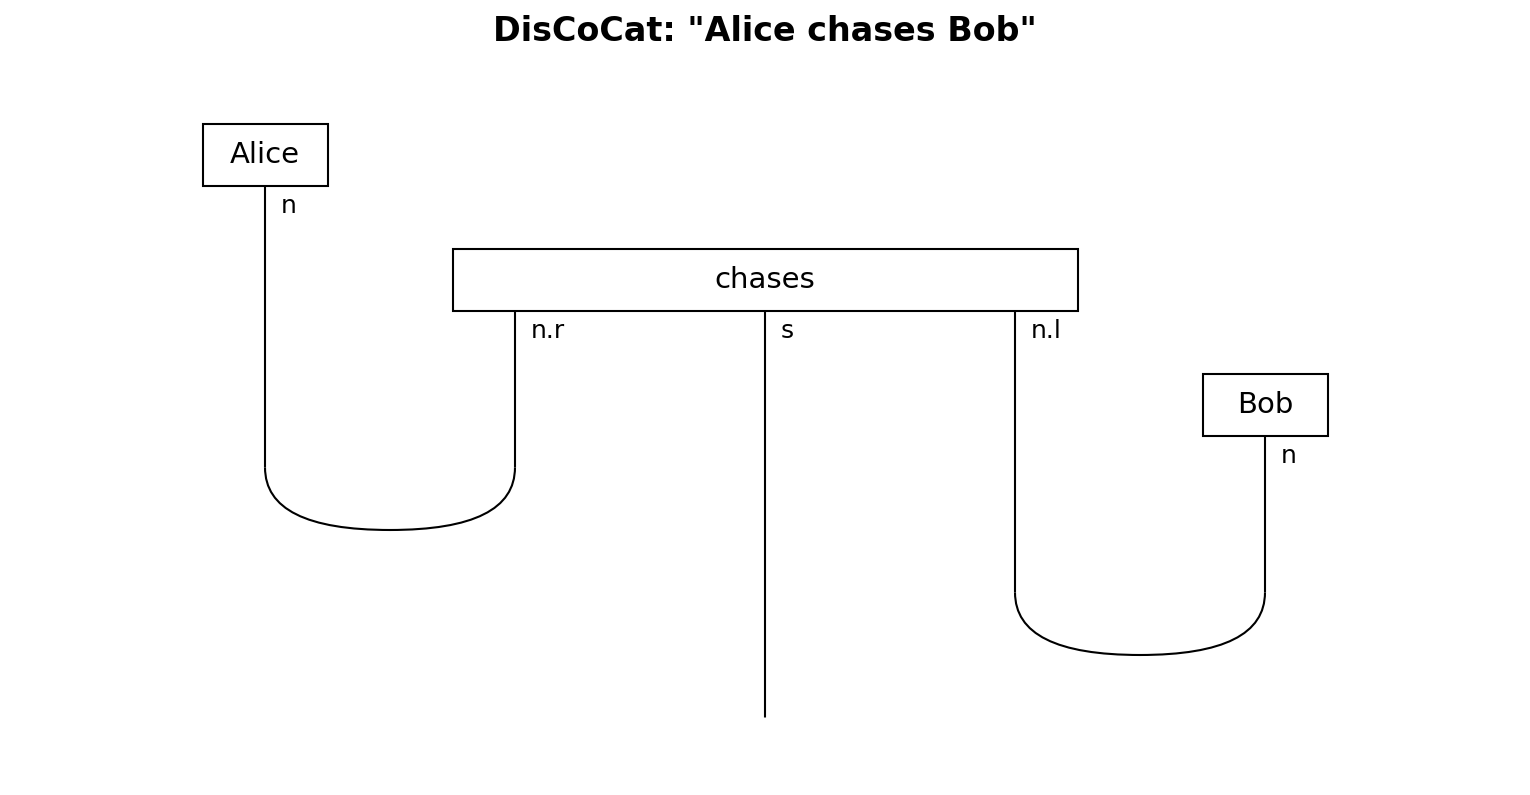
\includegraphics[keepaspectratio,alt={DisCoPy rendering of the DisCoCat sentence ``Alice chases Bob'' as a pregroup grammar string diagram, produced using the DisCoPy library's native drawing backend. The three Word boxes (Alice type n, chases type n.r @ s @ n.l, Bob type n) are connected by Cup contractions that cancel adjoint type pairs, reducing the entire expression to the sentence type s. This demonstrates the monoidal structure of type contraction that underlies all DisCoCat computations.}]{../figures/discopy_discocat.png}}
\caption{DisCoPy rendering of the DisCoCat sentence ``Alice chases Bob''
as a pregroup grammar string diagram, produced using the DisCoPy
library's native drawing backend. The three Word boxes (Alice type n,
chases type n.r @ s @ n.l, Bob type n) are connected by Cup contractions
that cancel adjoint type pairs, reducing the entire expression to the
sentence type s. This demonstrates the monoidal structure of type
contraction that underlies all DisCoCat
computations.}\label{fig:discopy-discocat}
\end{figure}
\end{block}
\end{frame}

\begin{frame}{Case Enrichment in the DisCoCat Framework}
\protect\phantomsection\label{case-enrichment-in-the-discocat-framework}
The present contribution lies in showing how case marking enriches the
DisCoCat framework with explicit role structure. In a case-marked
DisCoCat model:

\begin{enumerate}
\item
  \textbf{Typed noun spaces}: Instead of a single noun space \(N\), we
  define case-specific spaces
  \(N_{\text{NOM}}, N_{\text{ACC}}, N_{\text{DAT}}, \ldots\) Morphisms
  between these spaces encode case-changing operations (passivization,
  dative shift, etc.).
\item
  \textbf{Case-constrained composition}: The meaning functor \(F\) maps
  case-typed pregroup derivations to tensor contractions that respect
  case constraints. A verb seeking a nominative subject and accusative
  object contracts only with vectors from the appropriate spaces.
\item
  \textbf{Alignment as functor}: Cross-linguistic alignment differences
  correspond to different meaning functors. An accusative-language
  functor maps S and A arguments to the same noun space
  \(N_{\text{NOM}}\); an ergative-language functor maps S and P to a
  shared \(N_{\text{ABS}}\).
\end{enumerate}

\begin{figure}
\centering
\pandocbounded{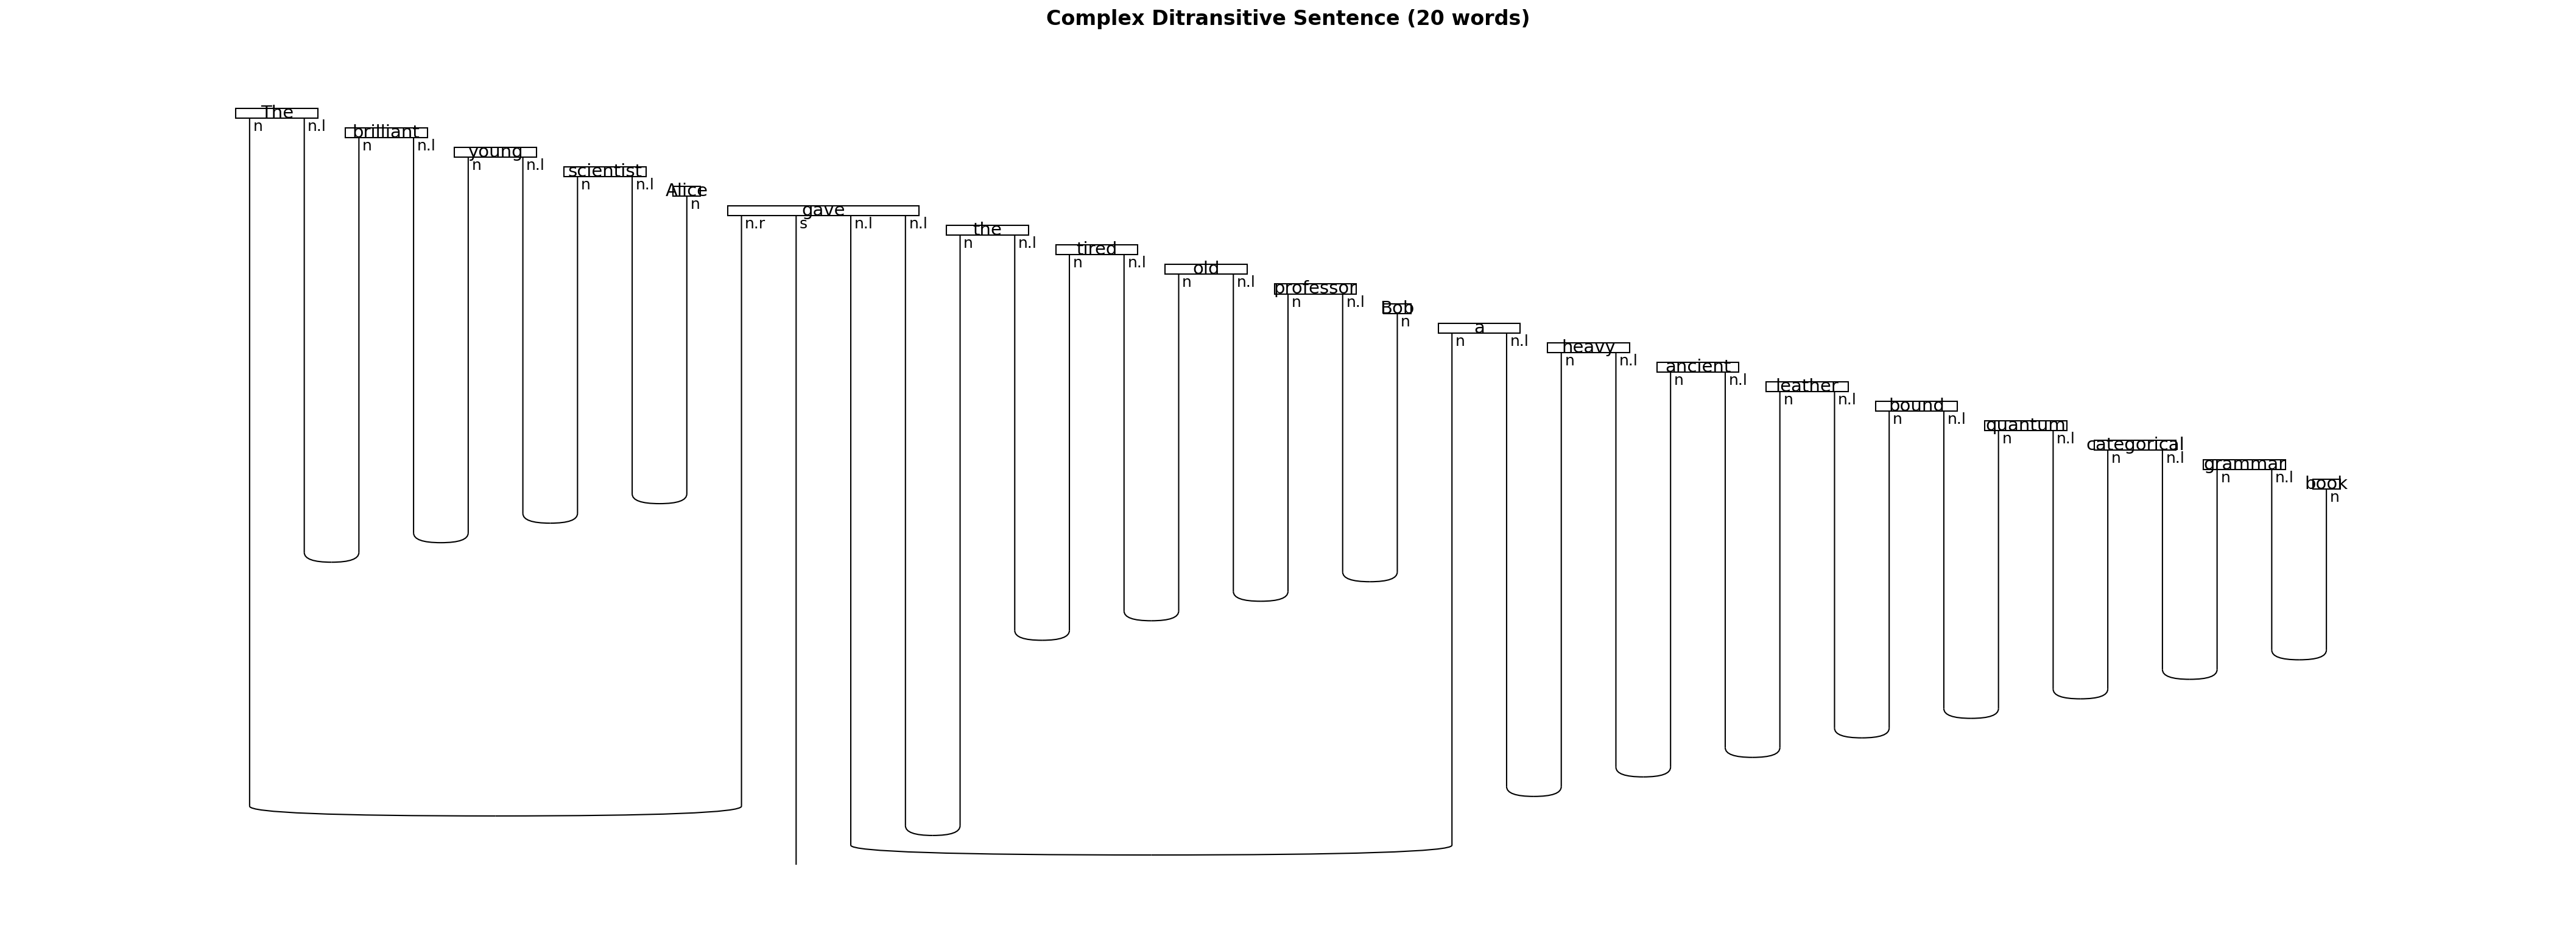
\includegraphics[keepaspectratio,alt={A massive 20-word DisCoPy pregroup grammar diagram for the complex ditransitive sentence ``The brilliant young scientist Alice gave the tired old professor Bob a heavy ancient leather bound quantum categorical grammar book.'' Generated entirely using DisCoPy's Python library, this tensor network demonstrates the combinatorial scalability of categorical compositional semantics. The diagram features three dense noun phrases (with 4, 4, and 8 chained adjective modifiers respectively), all reducing perfectly into the central verb's pregroup type n\^{}r \textbackslash otimes s \textbackslash otimes n\^{}l \textbackslash otimes n\^{}l. This single rigorous diagram maps 20 lexical items into a unified semantic type s, proving the empirical viability of string-diagrammatic grammar for complex natural language structures.}]{../figures/discopy_complex_sentence.png}}
\caption{A massive 20-word DisCoPy pregroup grammar diagram for the
complex ditransitive sentence ``The brilliant young scientist Alice gave
the tired old professor Bob a heavy ancient leather bound quantum
categorical grammar book.'' Generated entirely using DisCoPy's Python
library, this tensor network demonstrates the combinatorial scalability
of categorical compositional semantics. The diagram features three dense
noun phrases (with 4, 4, and 8 chained adjective modifiers
respectively), all reducing perfectly into the central verb's pregroup
type \(n^r \otimes s \otimes n^l \otimes n^l\). This single rigorous
diagram maps 20 lexical items into a unified semantic type \(s\),
proving the empirical viability of string-diagrammatic grammar for
complex natural language structures.}\label{fig:discopy-ditransitive}
\end{figure}
\end{frame}

\begin{frame}[fragile]{The Compact Closure Axiom and Diagrammatic
Complexity Metrics}
\protect\phantomsection\label{the-compact-closure-axiom-and-diagrammatic-complexity-metrics}
\begin{block}{The Snake Equation (Zigzag Identity)}
\protect\phantomsection\label{the-snake-equation-zigzag-identity}
The algebraic engine of DisCoCat is the \textbf{compact closure} of the
pregroup category: for every type \(n\), the adjunction maps
\(\eta_n: 1 \to n \otimes n^r\) (cap) and
\(\varepsilon_n: n^r \otimes n \to 1\) (cup) satisfy the \textbf{snake
equation} (also called the zigzag identity):

\[(\varepsilon_n \otimes 1_n) \circ (1_n \otimes \eta_n) = 1_n \tag{4.3}\]

In string-diagrammatic terms, a cup composed with a cap on adjacent
wires ``straightens out'' into an identity wire---a zigzag that cancels
into a straight line. This axiom is not merely a formal curiosity: it is
the \emph{engine} that makes pregroup type reductions work. Every
grammatical contraction (noun canceling with verb argument) is an
instance of the cup map \(\varepsilon\), and every expansion
(introducing an adjoint pair) is an instance of the cap map \(\eta\).
The snake equation guarantees that these contractions and expansions are
well-behaved---they can be freely inserted and removed without changing
the meaning of the derivation.

The cognitive significance of the snake equation is that it provides a
\emph{visual proof} of coherence: an agent inspecting a string diagram
can verify that the derivation is well-formed by checking that all
zigzags cancel---a spatial operation that requires no algebraic
computation. This is precisely Shimojima's
{[}-@shimojima1996reasoning{]} ``free ride'' in its purest form.

\begin{figure}
\centering
\pandocbounded{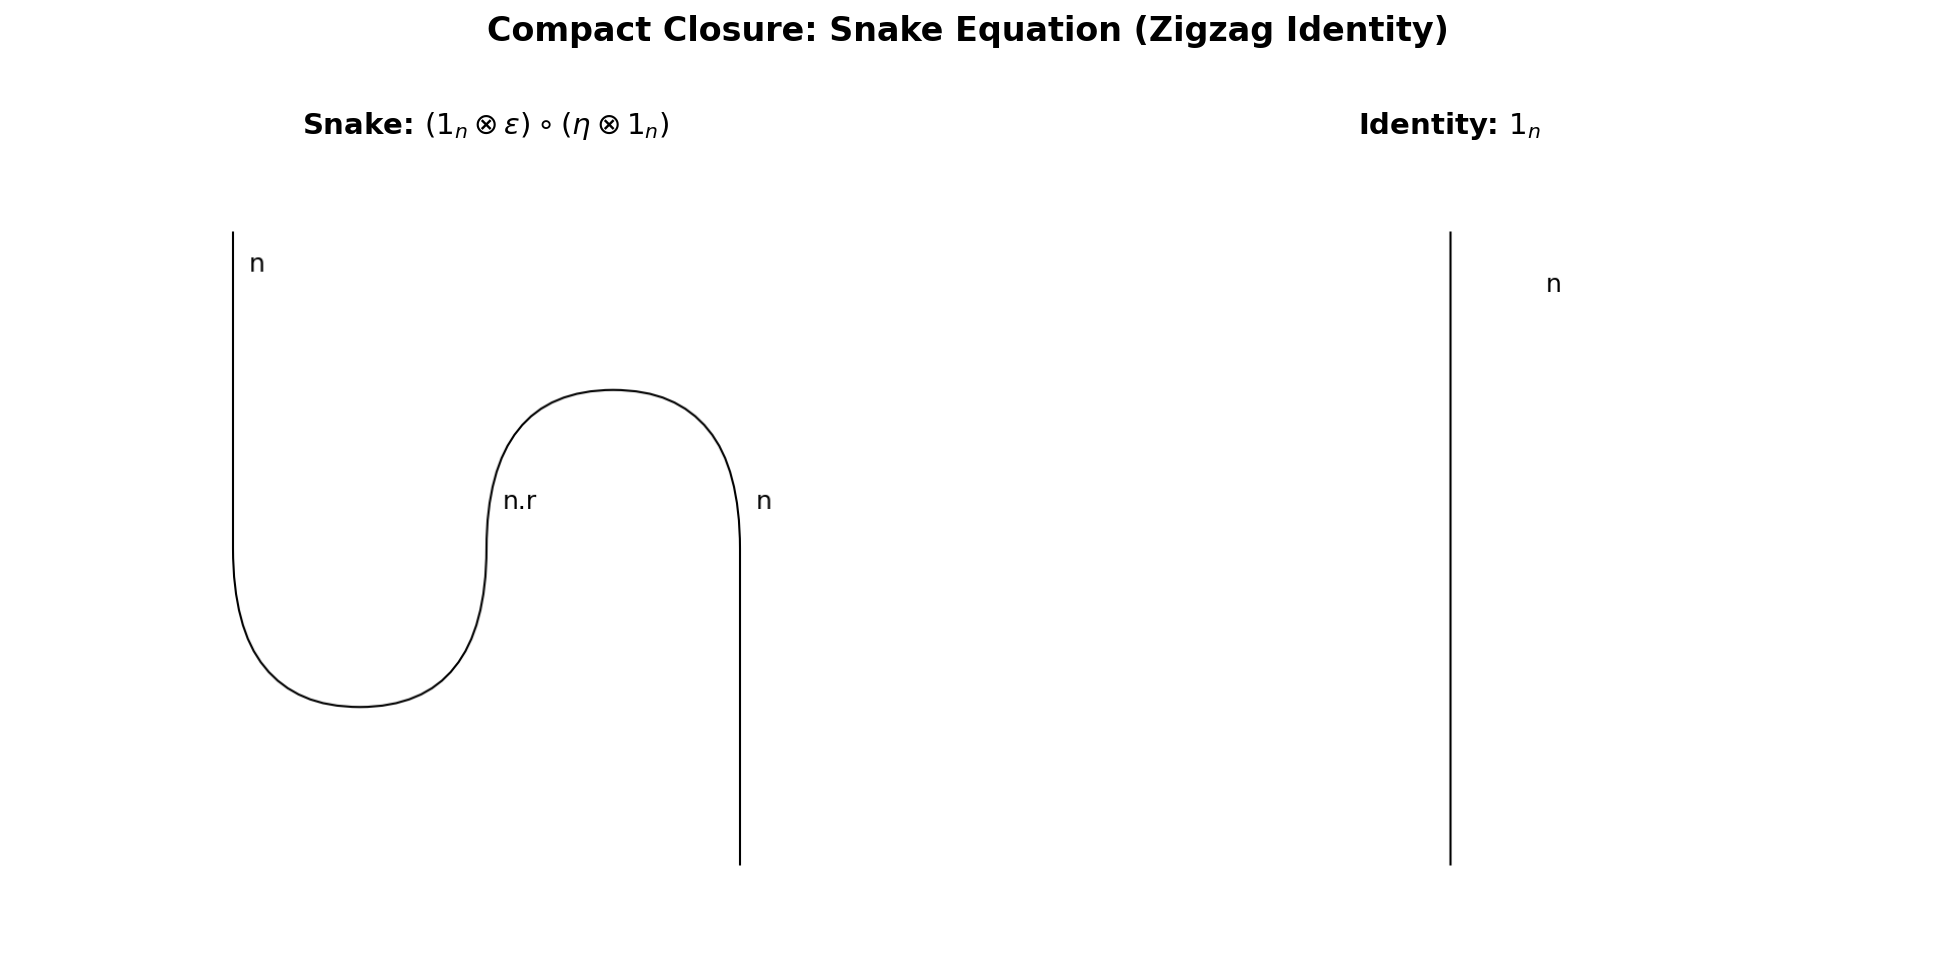
\includegraphics[keepaspectratio,alt={The snake equation (compact closure axiom) rendered by DisCoPy: the left panel shows the ``snake'' diagram where a Cup contraction (epsilon) composed with a Cap expansion (eta) on adjacent wires forms a zigzag; the right panel shows the identity wire it equals. This identity---that the zigzag straightens out---is the algebraic engine powering all pregroup type reductions and justifies the cancellation steps in every DisCoCat derivation.}]{../figures/discopy_snake.png}}
\caption{The snake equation (compact closure axiom) rendered by DisCoPy:
the left panel shows the ``snake'' diagram where a Cup contraction
(epsilon) composed with a Cap expansion (eta) on adjacent wires forms a
zigzag; the right panel shows the identity wire it equals. This
identity---that the zigzag straightens out---is the algebraic engine
powering all pregroup type reductions and justifies the cancellation
steps in every DisCoCat derivation.}\label{fig:discopy-snake}
\end{figure}
\end{block}

\begin{block}{Diagram Complexity Metrics: Normal Form and Depth}
\protect\phantomsection\label{diagram-complexity-metrics-normal-form-and-depth}
The algebraic properties of pregroup diagrams support quantitative
analysis of derivational complexity. Two measures are particularly
informative:

\begin{enumerate}
\item
  \textbf{Normal form}: A diagram is in \emph{normal form} if no further
  simplifications (zigzag cancellations, box reordering) are possible.
  The \texttt{normal\_form()} operation computes this canonical
  representative of the diagram's equivalence class.
\item
  \textbf{Depth}: The \emph{depth} of a diagram is the length of the
  longest path from input to output, counting boxes. Deeper diagrams
  encode more complex syntactic derivations---a ditransitive sentence
  like ``Alice gave Bob a book'' (depth 7) is structurally more complex
  than a simple intransitive ``Alice runs'' (depth 3).
\end{enumerate}

These metrics connect to the enriched framework of
\autoref{sec:enriched-categories}: the depth of a DisCoCat derivation
diagram can serve as a proxy for the syntactic complexity component of
the enriched hom-value, providing a principled bridge between the
type-logical and distributional perspectives on linguistic structure.
\end{block}
\end{frame}

\begin{frame}{Extensions: From Sentence Meaning to Discourse Coherence}
\protect\phantomsection\label{extensions-from-sentence-meaning-to-discourse-coherence}
\begin{block}{DisCoCirc: Distributional Compositional Circuits}
\protect\phantomsection\label{discocirc-distributional-compositional-circuits}
The original DisCoCat framework operates at the sentence level: each
sentence receives a vector meaning, but there is no mechanism for
tracking how meanings interact across sentences. De Felice and Coecke
{[}-@defelice2020discourse{]} address this with \textbf{DisCoCirc}
(Distributional Compositional Circuits), which extends the categorical
framework to handle discourse-level semantic structure.

DisCoCirc introduces \emph{state wires} that persist across sentence
boundaries, encoding the evolving states of discourse entities
(characters, objects, topics). A sentence like ``Alice chased Bob. He
was terrified.'' is represented as a circuit where:

\begin{itemize}
\tightlist
\item
  Alice and Bob are wires that persist across both sentences
\item
  The pronoun ``He'' is resolved by connecting its wire to Bob's wire
\item
  The emotional state ``terrified'' updates the state information
  carried by Bob's wire
\end{itemize}

De Felice et al. {[}-@defelice2022discocirc{]} further develop this into
a full-fledged circuit model that handles ambiguity, coreference, and
discourse coherence within the same categorical formalism. A CCG-based
pipeline for generating discourse circuits from syntactic parse trees
has recently demonstrated that DisCoCirc can scale to real-world text,
dynamically composing sentence-level diagrams along shared entity wires
via an iterative process of coreference resolution and wire merging
{[}-@duneau2021parsing{]}. Complementary work on \textbf{DiscoSG}
(Discourse Scene Graphs) extends this approach to multi-sentence image
captions, parsing text into scene graphs that capture cross-sentence
coreference relations. \autoref{fig:discourse} illustrates a
multi-sentence discourse diagram where entity wires persist across
sentence boundaries. For case theory, DisCoCirc is significant because
it shows how case-marked argument structure \emph{composes across
discourse}: the nominative subject of one sentence can become the
accusative object of the next, and this transformation is tracked as a
morphism in the discourse category.

\begin{figure}
\centering
\pandocbounded{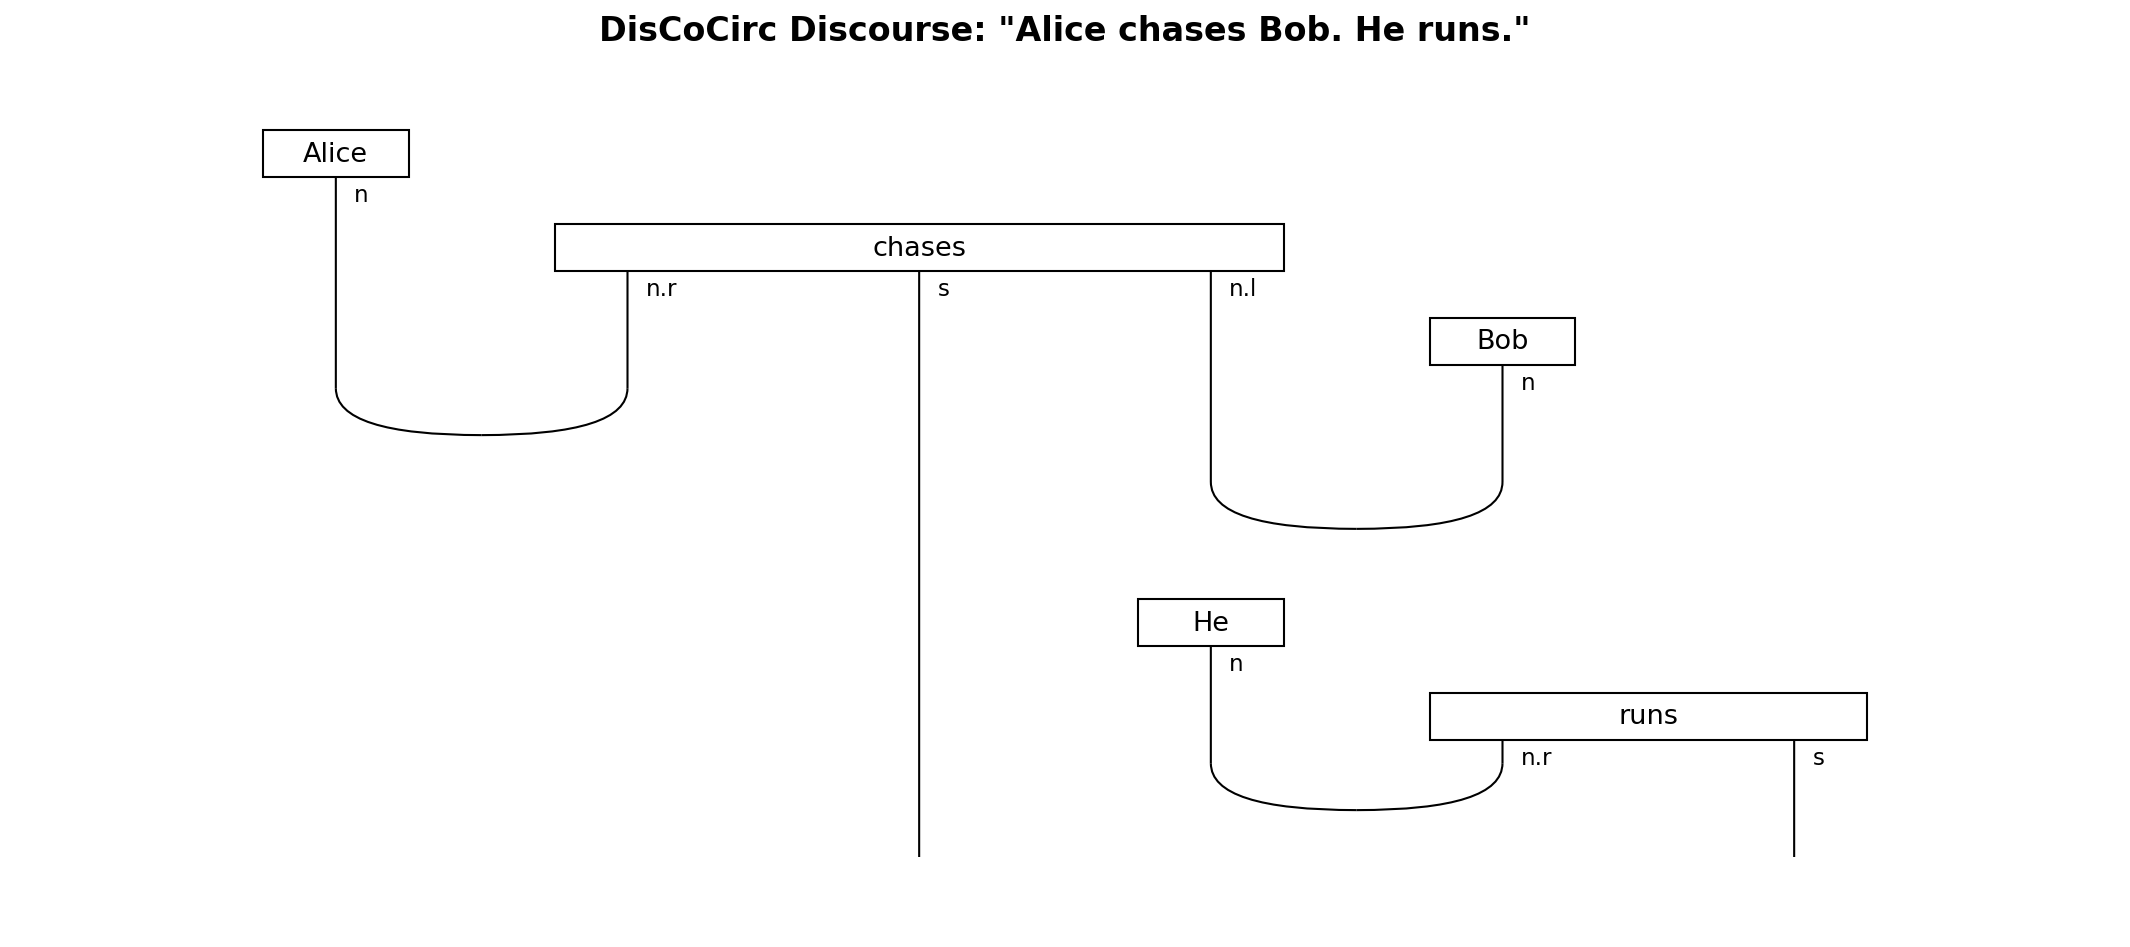
\includegraphics[keepaspectratio,alt={A DisCoCirc-style discourse diagram for the two-sentence discourse ``Alice chases Bob. Bob runs,'' generated using DisCoPy's pregroup grammar. Each sentence is rendered as a separate sub-diagram: Sentence 1 contracts Alice and Bob into the verb `chases' to produce sentence type s; Sentence 2 contracts Bob into `runs' to produce a second s. The full discourse is the tensor product s ⊗ s, encoding inter-sentential coherence through parallel compositional structure.}]{../figures/discopy_discocirc_discourse.png}}
\caption{A DisCoCirc-style discourse diagram for the two-sentence
discourse ``Alice chases Bob. Bob runs,'' generated using DisCoPy's
pregroup grammar. Each sentence is rendered as a separate sub-diagram:
Sentence 1 contracts Alice and Bob into the verb `chases' to produce
sentence type s; Sentence 2 contracts Bob into `runs' to produce a
second s. The full discourse is the tensor product s ⊗ s, encoding
inter-sentential coherence through parallel compositional
structure.}\label{fig:discourse}
\end{figure}
\end{block}

\begin{block}{Case Role Reversal Across Discourse Boundaries}
\protect\phantomsection\label{case-role-reversal-across-discourse-boundaries}
The power of DisCoCirc for case theory becomes particularly vivid in
multi-sentence discourses where the \emph{same entity occupies different
case roles} across sentences. Consider the three-sentence discourse:

\begin{quote}
\emph{``Alice chases Bob. Bob fears Alice. She smiles.''}
\end{quote}

In this discourse, Alice undergoes a complete cycle of case role
reversals:

\begin{enumerate}
\tightlist
\item
  \textbf{Sentence 1}: Alice is \(\text{NOM}\) (Proto-Agent, the one
  chasing) and Bob is \(\text{ACC}\) (Proto-Patient, the one chased).
\item
  \textbf{Sentence 2}: Bob is now \(\text{NOM}\) (the one fearing) and
  Alice is \(\text{ACC}\) (the one feared)---a role reversal where Alice
  moves from agent to patient.
\item
  \textbf{Sentence 3}: ``She'' resolves anaphorically to Alice, who
  returns to \(\text{NOM}\) as the agent of smiling.
\end{enumerate}

This NOM → ACC → NOM trajectory for Alice across three sentences is
precisely the kind of \emph{dynamic case assignment} that static
single-sentence analyses cannot capture. The categorical representation
as a triple tensor product \(s \otimes s \otimes s\)
(\autoref{fig:three-sentence-discourse}) encodes each sentence as an
independent pregroup derivation while preserving the entity identity
that links them. In a full DisCoCirc implementation, Alice's entity wire
would carry accumulated semantic state---the meaning of ``She'' in
sentence 3 inherits the enriched state of an Alice who has first chased
and then been feared, not merely the bare lexical entry for ``Alice.''

\begin{figure}
\centering
\pandocbounded{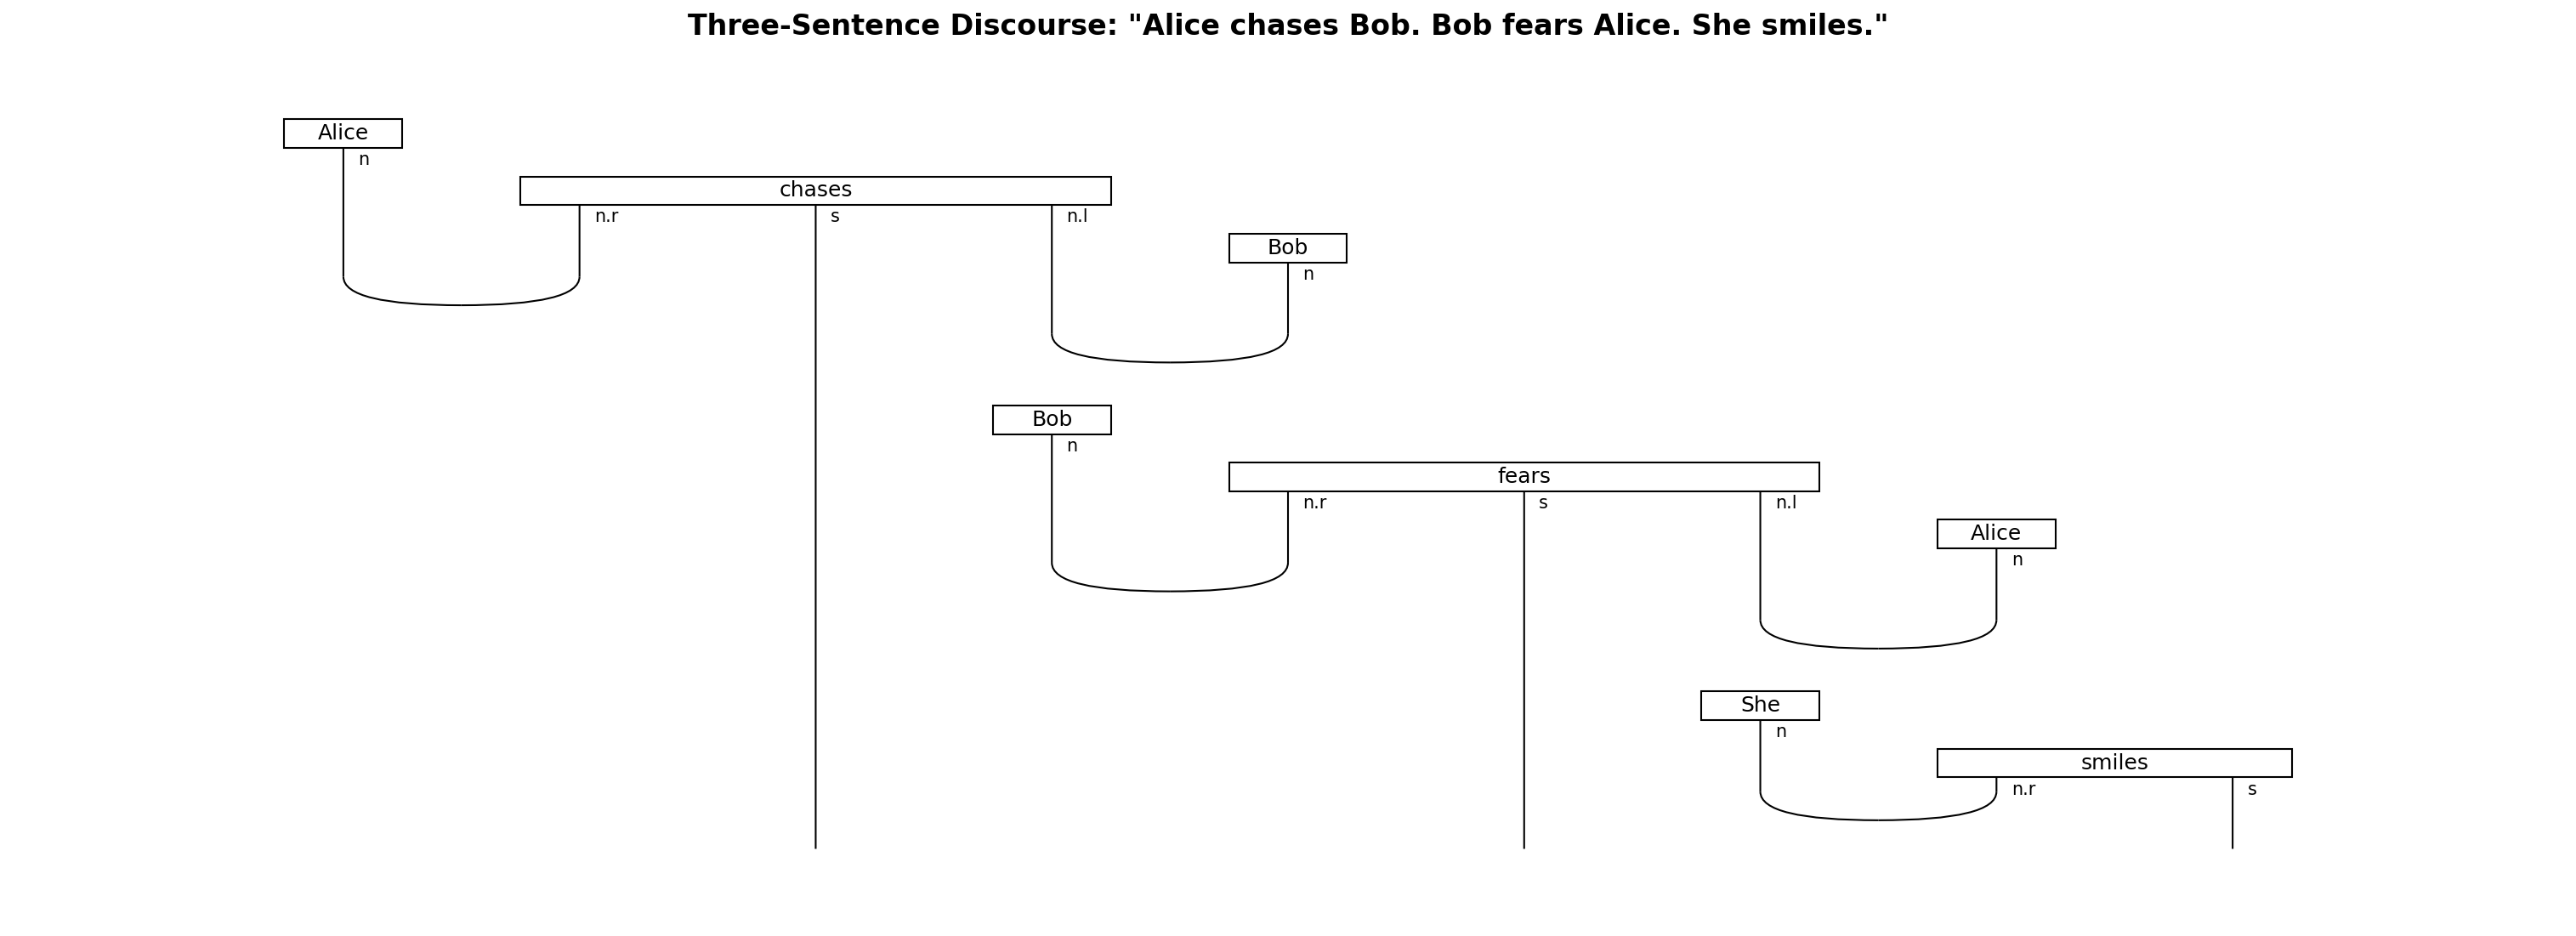
\includegraphics[keepaspectratio,alt={Three-sentence discourse diagram ``Alice chases Bob. Bob fears Alice. She smiles.'' rendered using DisCoPy's pregroup grammar. The diagram demonstrates case role reversal: Alice is NOM (agent) in sentence 1, ACC (patient) in sentence 2, and NOM again via the anaphoric pronoun ``She'' in sentence 3. Each sentence reduces independently to type s via cup contractions, and the full discourse is the triple tensor product s \textbackslash otimes s \textbackslash otimes s. This illustrates how DisCoCirc-style analyses track dynamic case assignment across discourse boundaries.}]{../figures/discopy_three_sentence_discourse.png}}
\caption{Three-sentence discourse diagram ``Alice chases Bob. Bob fears
Alice. She smiles.'' rendered using DisCoPy's pregroup grammar. The
diagram demonstrates case role reversal: Alice is NOM (agent) in
sentence 1, ACC (patient) in sentence 2, and NOM again via the anaphoric
pronoun ``She'' in sentence 3. Each sentence reduces independently to
type s via cup contractions, and the full discourse is the triple tensor
product \(s \otimes s \otimes s\). This illustrates how DisCoCirc-style
analyses track dynamic case assignment across discourse
boundaries.}\label{fig:three-sentence-discourse}
\end{figure}
\end{block}

\begin{block}{Quantum NLP and the lambeq Pipeline}
\protect\phantomsection\label{quantum-nlp-and-the-lambeq-pipeline}
The categorical structure of DisCoCat maps naturally onto quantum
circuits: the tensor product structure of \(\mathbf{FVect}\) is
identical to the tensor product structure of \(\mathbf{Qubit}\), the
category of qubit systems. This observation underlies the \textbf{QNLP}
(Quantum Natural Language Processing) program
{[}@meichanetzidis2020qnlp{]}, which implements DisCoCat models as
parameterized quantum circuits.

The \textbf{lambeq} library {[}@lorenz2023lambeq{]} provides a practical
pipeline:

\begin{enumerate}
\tightlist
\item
  Parse a sentence into a pregroup derivation
\item
  Convert the derivation into a string diagram
\item
  Translate the diagram into a parameterized quantum circuit (or a
  classical tensor network)
\item
  Train the parameters on NLP tasks (classification, similarity,
  question answering)
\end{enumerate}

Kartsaklis et al. {[}-@kartsaklis2021functorial{]} demonstrate that this
pipeline achieves competitive performance on question-answering tasks,
confirming that the categorical structure captures genuine linguistic
regularities even when instantiated on noisy near-term quantum hardware.

For our case-theoretic framework, QNLP offers a concrete computational
substrate: case categories could be implemented as quantum circuits
where case roles correspond to quantum registers and grammatical
relations correspond to parameterized gates. This connection between
linguistic case structure and quantum information processing---mediated
entirely by the shared categorical formalism---illustrates the power of
the diagrammatic approach.
\end{block}
\end{frame}

\end{document}
